%% abtex2-modelo-trabalho-academico.tex, v-1.9.6 laurocesar
%% Copyright 2012-2016 by abnTeX2 group at http://www.abntex.net.br/ 
%%
%% This work may be distributed and/or modified under the
%% conditions of the LaTeX Project Public License, either version 1.3
%% of this license or (at your option) any later version.
%% The latest version of this license is in
%%   http://www.latex-project.org/lppl.txt
%% and version 1.3 or later is part of all distributions of LaTeX
%% version 2005/12/01 or later.
%%
%% This work has the LPPL maintenance status `maintained'.
%% 
%% The Current Maintainer of this work is the abnTeX2 team, led
%% by Lauro César Araujo. Further information are available on 
%% http://www.abntex.net.br/
%%
%% This work consists of the files abntex2-modelo-trabalho-academico.tex,
%% abntex2-modelo-include-comandos and abntex2-modelo-references.bib
%%

% ------------------------------------------------------------------------
% ------------------------------------------------------------------------
% abnTeX2: Modelo de Trabalho Academico (tese de doutorado, dissertacao de
% mestrado e trabalhos monograficos em geral) em conformidade com 
% ABNT NBR 14724:2011: Informacao e documentacao - Trabalhos academicos -
% Apresentacao
% ------------------------------------------------------------------------
% ------------------------------------------------------------------------
%

\documentclass[
	% -- opções da classe memoir --
	12pt,				% tamanho da fonte
	openany,			% capítulos começam em pág ímpar (insere página vazia caso preciso)
  oneside,      % para impressão em página única. Oposto ao twoside (Nunca habilitar os dois!)
	%twoside,			% para impressão em recto e verso. Oposto a oneside (Nunca habilitar os dois!)
	a4paper,			% tamanho do papel. 
	% -- opções da classe abntex2 --
	%chapter=TITLE,		% títulos de capítulos convertidos em letras maiúsculas
	%section=TITLE,		% títulos de seções convertidos em letras maiúsculas
	%subsection=TITLE,	% títulos de subseções convertidos em letras maiúsculas
	%subsubsection=TITLE,% títulos de subsubseções convertidos em letras maiúsculas
	% -- opções do pacote babel --
	english,			% idioma adicional para hifenização
	french,				% idioma adicional para hifenização
	spanish,			% idioma adicional para hifenização
	brazil				% o último idioma é o principal do documento
	]{abntex2}

% ---
% Pacotes básicos 
% ---
\usepackage{lmodern}			  % Usa a fonte Latin Modern			
\usepackage[T1]{fontenc}		% Selecao de codigos de fonte.
\usepackage[utf8]{inputenc} % Codificacao do documento (conversão automática dos acentos)
\usepackage{lastpage}			  % Usado pela Ficha catalográfica
\usepackage{indentfirst}    % Indenta o primeiro parágrafo de cada seção.
\usepackage{color}				  % Controle das cores
\usepackage{graphicx}			  % Inclusão de gráficos
\usepackage{subfig}         % Sub-figuras
\usepackage{microtype}      % para melhorias de justificação
\usepackage{textcomp}       % Adiciona símbolo de trademark e outros ao T1
\usepackage{array}          % Usado nas tabelas com \newline
\usepackage{multirow}       % Define tabelas multirow
		
% ---
% Pacotes adicionais, usados apenas no âmbito do Modelo Canônico do abnteX2
% ---
\usepackage{lipsum}				% para geração de dummy text
% ---

% ---
% Pacotes de citações
% ---
\usepackage[brazilian,hyperpageref]{backref}	 % Paginas com as citações na bibl
\usepackage[alf]{abntex2cite}	% Citações padrão ABNT

% Copiado das configurações do LyX

%%%%%%%%%%%%%%%%%%%%%%%%%%%%%% LyX specific LaTeX commands.
%% Because html converters don't know tabularnewline
\providecommand{\tabularnewline}{\\}

%%%%%%%%%%%%%%%%%%%%%%%%%%%%%% User specified LaTeX commands.

% --- 
% CONFIGURAÇÕES DE PACOTES
% --- 

% ---
% Configurações do pacote backref
% Usado sem a opção hyperpageref de backref
\renewcommand{\backrefpagesname}{Citado na(s) página(s):~}
% Texto padrão antes do número das páginas
\renewcommand{\backref}{}
% Define os textos da citação
\renewcommand*{\backrefalt}[4]{
	\ifcase #1 %
		Nenhuma citação no texto.%
	\or
		Citado na página #2.%
	\else
		Citado #1 vezes nas páginas #2.%
	\fi}%
% ---

% --- 
% NOME DOS CLUSTERS 
% --- 

% ---
% Define o nome dos quatro clusters usados no trabalho.
\newcommand{\nomeCa}{Apaixonados}
\newcommand{\nomeCb}{Invejáveis}
\newcommand{\nomeCc}{Hamletianos}
\newcommand{\nomeCd}{Descomplicados}
% ---


% ---
% Informações de dados para CAPA e FOLHA DE ROSTO
% ---
\titulo{Consultoria A2IPG: Análise de Protótipos}
\autor{
  André Ferreira Bem Silva 
  \\
  Augusto Gonçalves
  \\
  Guilherme Borin
  \\
  Isadora Vieira
  \\
  Paola Villaça
}

\local{São Paulo, SP}
\data{29/09/2017}
%\coorientador{}
\instituicao{%
  Fundação Getúlio Vargas -- FGV
  \par
  MBA Executivo em Economia e Gestão: Business Analytics e Big Data T3
  \par
  Disciplina de Inferência Estatística
}
\tipotrabalho{Relatório Final}
% O preambulo deve conter o tipo do trabalho, o objetivo, 
% o nome da instituição e a área de concentração 
\preambulo{Este trabalho trata-se de uma possível consultoria acerca da amostra de entrevistas quanto a protótipos de carros, adaptada de uma amostra real do carro Ford Ka\texttrademark}
% ---


% ---
% Configurações de aparência do PDF final

% alterando o aspecto da cor azul
\definecolor{blue}{RGB}{41,5,195}

% informações do PDF
\makeatletter
\hypersetup{
     	%pagebackref=true,
		pdftitle={\@title}, 
		pdfauthor={\@author},
    	pdfsubject={\imprimirpreambulo},
	    pdfcreator={LaTeX with abnTeX2},
		pdfkeywords={abnt}{latex}{abntex}{abntex2}{trabalho acadêmico}, 
		colorlinks=true,       		% false: boxed links; true: colored links
    	linkcolor=blue,          	% color of internal links
    	citecolor=blue,        		% color of links to bibliography
    	filecolor=magenta,      		% color of file links
		urlcolor=blue,
		bookmarksdepth=4
}
\makeatother
% --- 

% --- 
% Espaçamentos entre linhas e parágrafos 
% --- 

% O tamanho do parágrafo é dado por:
\setlength{\parindent}{1.3cm}

% Controle do espaçamento entre um parágrafo e outro:
\setlength{\parskip}{0.2cm}  % tente também \onelineskip

% ---
% compila o indice
% ---
\makeindex
% ---

% ----
% Início do documento
% ----
\begin{document}

% Seleciona o idioma do documento (conforme pacotes do babel)
%\selectlanguage{english}
\selectlanguage{brazil}

% Retira espaço extra obsoleto entre as frases.
\frenchspacing 

% ----------------------------------------------------------
% ELEMENTOS PRÉ-TEXTUAIS
% ----------------------------------------------------------
% \pretextual

% ---
% Capa
% ---
\imprimircapa
% ---

% ---
% Folha de rosto
% (o * indica que haverá a ficha bibliográfica)
% ---
\imprimirfolhaderosto
% ---

% ---

% ---

% ---

% ---
% inserir lista de ilustrações
% ---
%\pdfbookmark[0]{\listfigurename}{lof}
\listoffigures*
%\cleardoublepage
% ---

% ---
% inserir lista de tabelas
% ---
\pdfbookmark[0]{\listtablename}{lot}
\listoftables*
% ---

% ---
% inserir lista de abreviaturas e siglas
% ---
%\begin{siglas}
%  \item[ABNT] Associação Brasileira de Normas Técnicas
%  \item[abnTeX] ABsurdas Normas para TeX
%\end{siglas}
% ---

% ---
% inserir lista de símbolos
% ---
%\begin{simbolos}
%  \item[$ \Gamma $] Letra grega Gama
%  \item[$ \Lambda $] Lambda
%  \item[$ \zeta $] Letra grega minúscula zeta
%  \item[$ \in $] Pertence
%\end{simbolos}
% ---

% ---
% inserir o sumario
% ---
\pdfbookmark[0]{\contentsname}{toc}
\tableofcontents*
\cleardoublepage
% ---



% ----------------------------------------------------------
% ELEMENTOS TEXTUAIS
% ----------------------------------------------------------
\textual

% ----------------------------------------------------------
% Introdução (exemplo de capítulo sem numeração, mas presente no Sumário)
% ----------------------------------------------------------
%\chapter*[Introdução]{Introdução}
%\addcontentsline{toc}{chapter}{Introdução}
% ----------------------------------------------------------

%Adiciona introdução com numeração
\chapter[Introdução]{Introdução}
% Adiciona o arquivo de analise de p-valor (Augusto)
\section{Objetivo}

%Somos o banco X e vamos decidir se emprestamos ou não para o cliente Y (no nosso caso para a Positivo Informática S/A)
Por meio de uma análise detalhada e consolidada dos indicadores da empresa \nomeCompletoPositivo{}, define-se o risco de investimento na mencionada empresa por parte do \emph{\nomeDoBanco{}}. Sendo assim, essa análise deve definir, seguindo métricas e métodos de controladoria gerencial, uma recomendação ao \emph{board} do banco para que possam tomar uma decisão referente ao mesmo.

\section{Risco de Crédito}

\section{Histórico}
A Positivo Tecnologia nasceu do Grupo Positivo, que é o maior grupo do segmento de educação no Brasil. Fundado em 1972, a partir da criação de uma escola e de uma gráfica, o Grupo Positivo possui atualmente empresas líderes nos três segmentos em que atua: educacional, gráfico-editorial e tecnologia. A partir do grande sucesso de sua inovadora metodologia de ensino desenvolvida, aprimorada e sistematizada pelos conceituados professores fundadores do grupo, a rede de escolas próprias foi ampliada para os demais níveis educacionais e, em 1979, o grupo iniciou a venda de livros e serviços a outras escolas em todo Brasil.

Em 1989, os mesmos empreendedores do grupo iniciaram a produção de computadores pessoais, criando assim a Positivo Informática. Inicialmente, este ramo do grupo focou apenas na produção e comercialização de computadores para escolas clientes do Grupo Positivo em todo o Brasil. Atualmente, no ramo de tecnologia, a empresa produz computadores, laptops, tablets, smartphones, celulares e, mais recentemente, dispositivos de telemedicina. 

A semente original do grupo ainda se mantém, o grupo conta com cerca de 27 mil alunos em suas unidades próprias (Escolas Positivo, Curso Positivo e Universidade Positivo), além de ter atendido a aproximadamente 10 milhões de alunos com seus produtos e serviços desde sua fundação. Os Portais Educacionais do Grupo Positivo estão presentes em cerca de 11,0 mil escolas. Além disso, a Posigraf é a primeira gráfica Carbono Zero do país. O Grupo Positivo conta atualmente com mais de 9,0 mil colaboradores.

\section{Perfil Corporativo}

\begin{figure}[h]
\begin{centering}
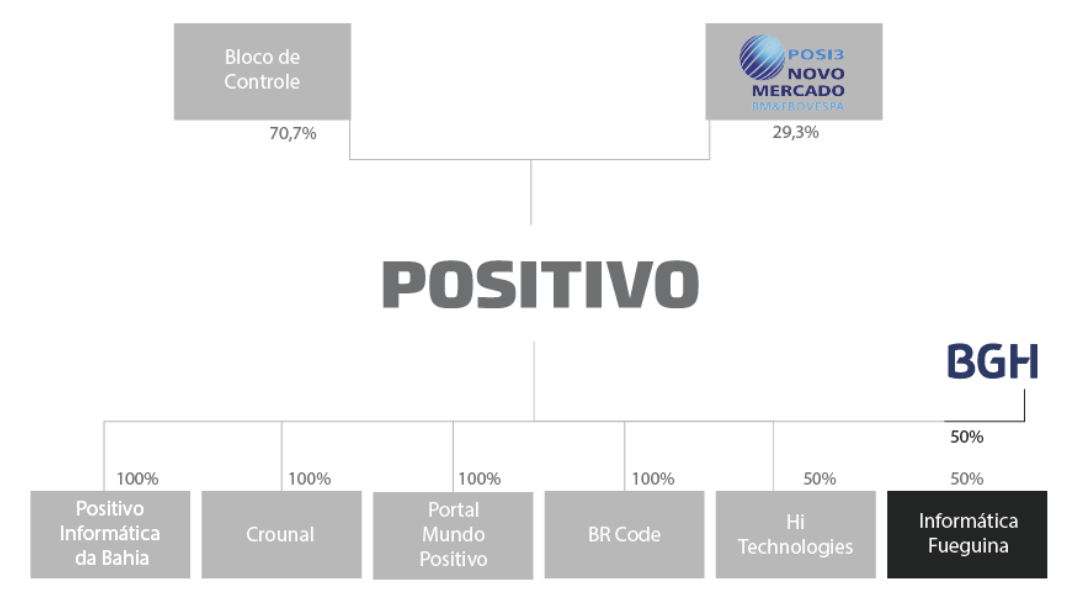
\includegraphics[width=1.0\textwidth]{Img/Corporativo}
\caption{Figura que demonstra o domínio e capital social da \nomeCompletoPositivo{}.}
\par\end{centering}
\end{figure}

Em 2016, a Positivo Tecnologia foi uma das maiores fabricantes de computadores no Brasil, respondendo por 15,3\% do número total de computadores vendidos no mercado brasileiro, de acordo com a IDC. No mesmo período, obtiveram uma participação de 19,9\% do mercado de varejo. Uma parcela substancial da produção de computadores é vendida através de grandes redes de varejo, com as quais o grupo mantém sólido relacionamento comercial, em função principalmente dos preços competitivos, do reconhecimento da marca e assistência técnica.

Adicionalmente, a companhia atua no mercado argentino por meio da marca \nomePositivoAr{}, fruto de uma joint venture com um parceiro local. Em 2015, os computadores \nomePositivoAr{} atingiram uma participação de 9,5\%, segundo a IDC.

No Brasil, a Positivo Tecnologia oferece uma linha completa de dispositivos, incluindo computadores de mesa (desktops e all-in-ones), computadores portáteis (notebooks e netbooks) e tablets, que são produzidos em Manaus (AM). Em 2012, a Companhia ingressou no mercado de telefones celulares, com a oferta de smartphones e messaging phones.

\begin{figure}[h]
\begin{centering}
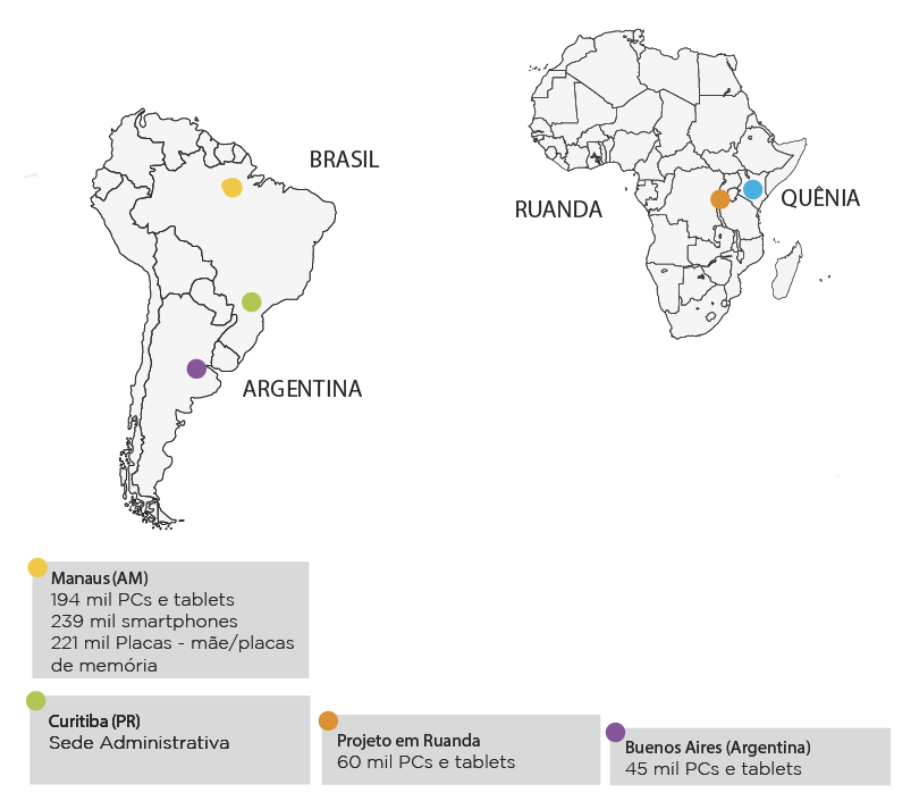
\includegraphics[width=1.0\textwidth]{Img/PositivoMundo}
\caption{Operações da \nomePositivo{} a nível mundial, bastante expressiva na América Latina e observa-se também sítios na África.}
\par\end{centering}
\end{figure}

Além disso, para atendimento e suporte aos milhões de consumidores finais, empresas e órgãos do governo, conta com uma ampla e capacitada rede de assistências técnicas cobrindo a totalidade do território nacional, e com a CRP - Central de Relacionamento Positivo, que registrou em média, 2,9 mil contatos diários em 2016. Grande parte destes contatos se refere a questões básicas sobre uso do computador, sistema operacional ou problemas com conexões, uma vez que muitos dos clientes estão adquirindo seu computador pela primeira vez.

Parcela menor da receita da Companhia provém do Segmento de Tecnologia Educacional, no qual acredita ser líder absoluto no País. A Companhia oferece soluções de infraestrutura e gestão, aplicativos e plataformas educacionais, portais de educação, além de formação de professores e acompanhamento pedagógico. Os portais têm mais de 1,2 milhões de usuários ativos, com modelo de receita recorrente mensal. 

As soluções educacionais da Positivo Tecnologia estão presentes em mais de 14 mil escolas e são exportadas para mais de 40 países. Dentre os principais produtos estão mesas educacionais, dispositivos móveis, lousas interativas, dispositivos de armazenamento e recarga, projetores, acess point, e sistema de gerenciamento de aulas. A Companhia é também distribuidor exclusivo no Brasil de empresas líderes no desenvolvimento e distribuição de software educacional, bem como distribui produtos da LEGO\texttrademark Education no território nacional.

Em 2016, a Companhia ingressou no mercado de tecnologia médica por meio da aquisição de 50\% do capital social da Hi Technologies S.A., empresa com forte foco em P\&D para a oferta de produtos inovadores em saúde.


% ----------------------------------------------------------
% Análise dos clusters
% ----------------------------------------------------------

\chapter{Análise de Clusters}
\label{chap:analise}
Conforme identificado no capítulo \ref{chap:introducao}, em posse
dos dados, devemos classificá-los de forma a identificar os diferentes
segmentos de mercado na população, verificar para quais desses segmentos
o produto é mais interessante e direcionar a comunicação e criar a
campanha de marketing de forma a atingir essa parte da população.

A ferramenta de análise utilizada para resolução desse problema será
a Análise de Cluster, também conhecida como análise de conglomerados.

A análise de cluster é uma técnica de análise multivariada cujo principal
objetivo é reunir pontos de dados baseando-se nas características
individuais de cada um. Ou seja, ele classifica cada elemento segundo
aquilo que cada um tem de similar em relação a outros pertencentes
a um determinado grupo, considerando um critério de seleção predeterminado.

O resultado da Análise de Cluster deve exibir um alto grau de homogeneidade
interna (dentro do cluster) e alto grau de heterogeneidade externa
(entre os diferentes clusters) conforme demonstrado na figura \ref{fig:clustering}.

\begin{figure}
\begin{centering}
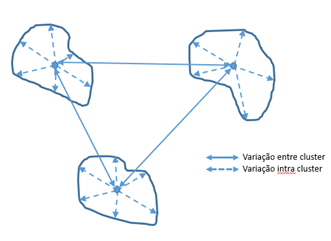
\includegraphics[width=0.65\textwidth]{Imagens/clustering}
\par\end{centering}

\caption{\label{fig:clustering}Heterogeneidade e homogeneidade}
\end{figure}


Esse tipo de análise é utilizada em diferentes campos de estudo, como
psicologia, biologia, marketing, engenharia, administração e contabilidade.
Entretanto em todos esses campos a análise tem um objetivo comum.
Classificar os elementos de acordo com os relacionamentos naturais.

Existem diferentes maneiras e técnicas de se aplicar esse tipo de
análise, em nosso caso será utilizado o método de Ward, que é um método
no qual a soma dos quadrados dos desvios de cara elemento em relação
a cada conglomerado é minimizada. Esse método tem uma tendência a
combinar grupos com um menor número de observações e produz grupos
com aproximadamente o mesmo número de elementos.

Por fim, ao final da análise deve-se interpretar os resultados, o
que envolve o exame de cada grupo levando em conta o conjunto de variáveis
eleitas para atribuir uma identificação que descreva adequadamente
a natureza dos grupos.

No caso estudado a análise de cluster mostra-se especialmente útil
pois ela classifica os elementos em diferentes segmentos de mercado
e auxilia na escolha de qual protótipo seria mais indicado a cada
grupo, bem como indicaria qual o tipo de comunicação deveria ser feita
a cada grupo após escolhido o protótipo.

\begin{figure}
\begin{centering}
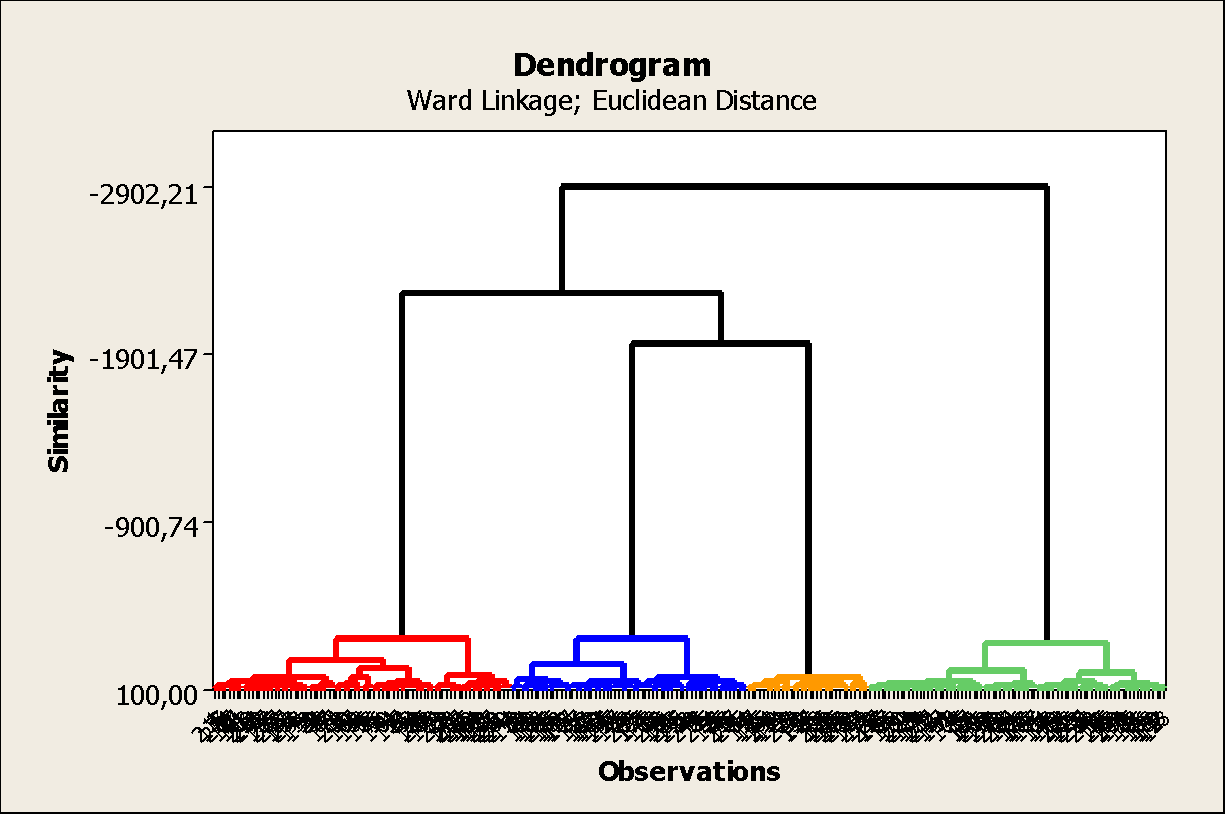
\includegraphics[width=0.85\textwidth]{Imagens/dendogram}
\par\end{centering}

\caption{\label{fig:dendogram}O Dendograma por método de Ward tomados \emph{Imagem,
Utilitário e Preço}.}
\end{figure}


\begin{table}
\begin{centering}
\begin{tabular}{c|c|c|c|c|c}
\hline 
Variável & Cluster 1 & Cluster 2 & Cluster 3 & Cluster 4 & Centróide\tabularnewline
\hline 
Imagem & 2,35 & 3,04 & 0,95 & 0,62 & 2,00\tabularnewline
\hline 
Utilitário & 2,95 & 1,57 & 0,99 & 3,47 & 2,10\tabularnewline
\hline 
Preço & 2,89 & 0,98 & 2,36 & 0,54 & 1,86\tabularnewline
\hline 
\end{tabular}
\par\end{centering}

\caption{\label{tab:centroids-ward}Centróides de clustering obtidos por método
de Ward}
\end{table}


O dendograma apresentado na figura \ref{fig:dendogram} e na tabela
\ref{tab:centroids-ward} denotam a relação entre \emph{Imagem, Preço,
Utilitário }e\emph{ Cluster }que é usada como base na abordagem de
\emph{Persona }neste capítulo. Na tabela, observa-se uma atração do
cluster 1 para \emph{Imagem}, \emph{Utilitário} e \emph{Preço}. Do
cluster 2 para \emph{Imagem}, do 3 para \emph{Preço} e do 4 para \emph{Utilitário}.



% Adiciona o arquivo de analise de p-valor (Paola)
\section{Personas}

A análise de personas, a nível de marketing, é um perfil semifictício
que representa um estereótipo de cliente da empresa. Na análise de
protótipos, definimos uma persona por cluster para que assim possamos
melhor caracterizá-los. Nas próximas seções são definidos uma persona
por cluster.


\subsection{Cluster 1: Persona \nomeCa{}}

Pedro 30 anos advogado bem-sucedido admite sua paixão por carro. Para
ele o carro é um objeto de desejo que diz quem você é, representa
a passagem para um futuro cada vez mais avançado, além de trazer agilidade
no dia-a-dia e conforto nas viagens. 

\subsubsection{Preferência}
Mostrou que dentre os quatro clusters analisados, este é o mais heterogêneo,
porém analisando o cruzamento com as três variáveis psicográficas
foi o que mostrou maior interesse em todas elas, e o preço foi a variável
mais relevante. Para estas pessoas o carro reflete a sua imagem, é
visto como um bem utilitário e o preço precisa obrigatoriamente dar
um retorno em relação à expectativa que eles possuem quanto a imagem
e a tecnologia. São pessoas que conhecem carro, não se importam em
pagar caro, desde que tenham os benefícios, isto é, o carro seja realmente
uma máquina bela e possante. 


\subsection{Cluster 2: Persona \nomeCb{}}

Marcelo executivo de sucesso 55 anos, seu carro é a sua própria imagem.
Segundo ele, dependendo do modelo, que varia com os anseios de cada
um, o carro transmite a mensagem que seu dono pode ser ou forte, ou
livre, ou rico, ou aventureiro, ou ter todas, ou algumas dessas características.
Um carro limpo e brilhante está associado ao sucesso social, à estabilidade
financeira e ao cuidado com seus pertences. 

\subsubsection{Preferência}
É possível concluir que este cluster é bem homogêneo. A análise
do cruzamento do cluster com as variáveis psicográficas mostrou que
o maior peso foi dado à variável imagem, e as variáveis utilitário
e preço tiveram igualmente um peso bem menor. Isso significa que as
pessoas que fazem parte deste cluster estão dispostas a pagar o preço
que for por um carro que traduza fielmente o que pretendem transmitir
a sociedade. Não estão preocupadas com o que o carro oferece de utilitários
nem mesmo com a relação custo-benefício, o fator de escolha é apenas
a imagem transmitida pelo bem. 


\subsection{Cluster 3: Persona \nomeCc{} }

Clara é uma jovem estudante preocupada com a preservação
do planeta, com o clima, com a ameaça do fim dos recursos naturais.
Para ela a sociedade deve se preocupar em diminuir o nível de consumo
e criar alternativas de consumo coletivo, compartilhamento de bens.
Ela se questiona se é recomendável comprar um carro. 

\subsubsection{Preferência}
Bem heterogêneo. O cruzamento das variáveis cluster e imagem demonstrou que existe
uma relação entre elas, porém o peso dado é menor comparado aos outros
clusters. Analisando o cruzamento das variáveis cluster e utilitário,
verificou-se que o peso dado foi menor ainda. A variável preço foi
a que obteve o maior peso. Estas pessoas demonstram ser indiferentes
a ter um carro, para elas a imagem que ter um carro transmite não
importa, e o carro como utilitário também não. Se comprassem um carro,
o preço seria um fator de escolha em detrimento da imagem e da utilidade. 

\subsection{Cluster 4: Persona \nomeCd{} }

Mariana é médica e tem dois filhos, sua vida é muito corrida pois
precisa conciliar o trabalho com a rotina dos filhos. Para ela, o
carro fez com que nos tornássemos \textquotedblleft auto-móveis\textquotedblright .
O carro nada mais é do que um bem utilitário, e quando ele deixa de
ser adequado às suas necessidades práticas, não lhe parece tão doloroso
trocá-lo por outro. Ela quer um produto seguro e, de preferência,
fácil de estacionar. 

\subsubsection{Preferência}
Este cluster é o mais homogêneo dentre os quatro. As pessoas que fazem
parte deste cluster valorizam o carro como utilitário mais do que
as pessoas dos outros três clusters. No cruzamento das variáveis cluster
e imagem, e cluster e preço, foi possível verificar que estas variáveis
receberam igualmente menor peso dentro do cluster, e em relação aos
outros clusters também. Este cluster vê o carro somente como um bem
utilitário, não criam nenhum tipo de apego afetivo, e trocam quando
não lhe serve mais. 


% Adiciona o arquivo de analise de p-valor (André)
\section{Análise das \emph{p}-variáveis para os Clusters}

Tendo em vista o dendograma da figura \ref{fig:dendogram} e a visualização dos
clusters na \ref{fig:clustering}, a análise das \emph{p}-variáveis é um método
de discriminação de quais elementos são contundentes na seleção do protótipo,
dados os clusters em questão. 

Nesta seção, vamos discorrer sobre as diversas variáveis do espaço
amostral e sua relação com os clusters \emph{\nomeCa{}}, \emph{\nomeCb{}}, \emph{\nomeCc{}}
e \emph{\nomeCd{}}.
\begin{table*}
\begin{centering}
\begin{tabular}{c|c|c|c|c|c}
\hline 
Protótipo/Cluster & \nomeCa{} & \nomeCb{} & \nomeCc{} & \nomeCd{} & Todos\tabularnewline
\hline 
1 & 51,28 & 2,56 & 3,23 & 87,5 & 28,80\tabularnewline
\hline 
2 & 37,18 & 5,13 & 93,55 & 0 & 36,40\tabularnewline
\hline 
3 & 11,54 & 92,31 & 3,23 & 12,5 & 34,80\tabularnewline
\hline 
\emph{Total} & 100 & 100 & 100 & 100 & 100\tabularnewline
\hline 
\end{tabular}
\par\end{centering}

\caption{\label{tab:prototipo-vs-cluster}Tabela de Análise Chi-quadrado ($\chi^{2}=281,52$;$DF=6$)
Protótipo x Cluster. Valor $p=0$.}
\end{table*}

\subsection{Protótipo}

Na tabela \ref{tab:prototipo-vs-cluster}, fica explícito a relação
entre variáveis protótipo e os clusters distintos. O protótipo 1 é
preferido entre os clusters \emph{\nomeCa{}} e \emph{\nomeCd{}},
o protótipo 2 no cluster \emph{\nomeCc{}} e o protótipo 3 no \emph{\nomeCb{}}.

Logo vê-se que os \emph{\nomeCa{}} fazem jus ao seu pseudônimo, apresentando
um comportamento bem heterogêneo em relação aos protótipos. Ainda
assim, concentram-se mais no 1 e no 2, cujas características estão
mais alinhadas com as observadas no cluster. 

É possível que para esse cluster somente uma estratégia de marketing
não seja o suficiente, concluindo que sem dúvidas esse é o cluster
mais desafiador da amostra analisada.

Já o cluster \emph{\nomeCc{}} é caracterizado pela inexistência de
um interesse específico no carro que não o preço, este é considerado
o cluster mais improvável para uma propaganda estratégica e de marketing,
sendo assim imediatamente descartado para tal fim. Isto é, nem uma
estratégia de marketing transformativo e nem informativo serão eficazes
tratando-se da população desse cluster.

O protótipo 3 apresenta forte correlação com os \emph{\nomeCb{}},
constituindo-se no segundo mais homogêneo com relação ao protótipo.
É possível que a característica mais associada a imagem do cluster
em questão influencie nessa escolha? 
\begin{figure}[h]
\begin{centering}
\subfloat[\label{fig:cluster-vs-preco}Cluster vs Preço: Teste One-way ANOVA
indica $p=0$ e $R_{adj}=85,47\%$.]{\begin{centering}
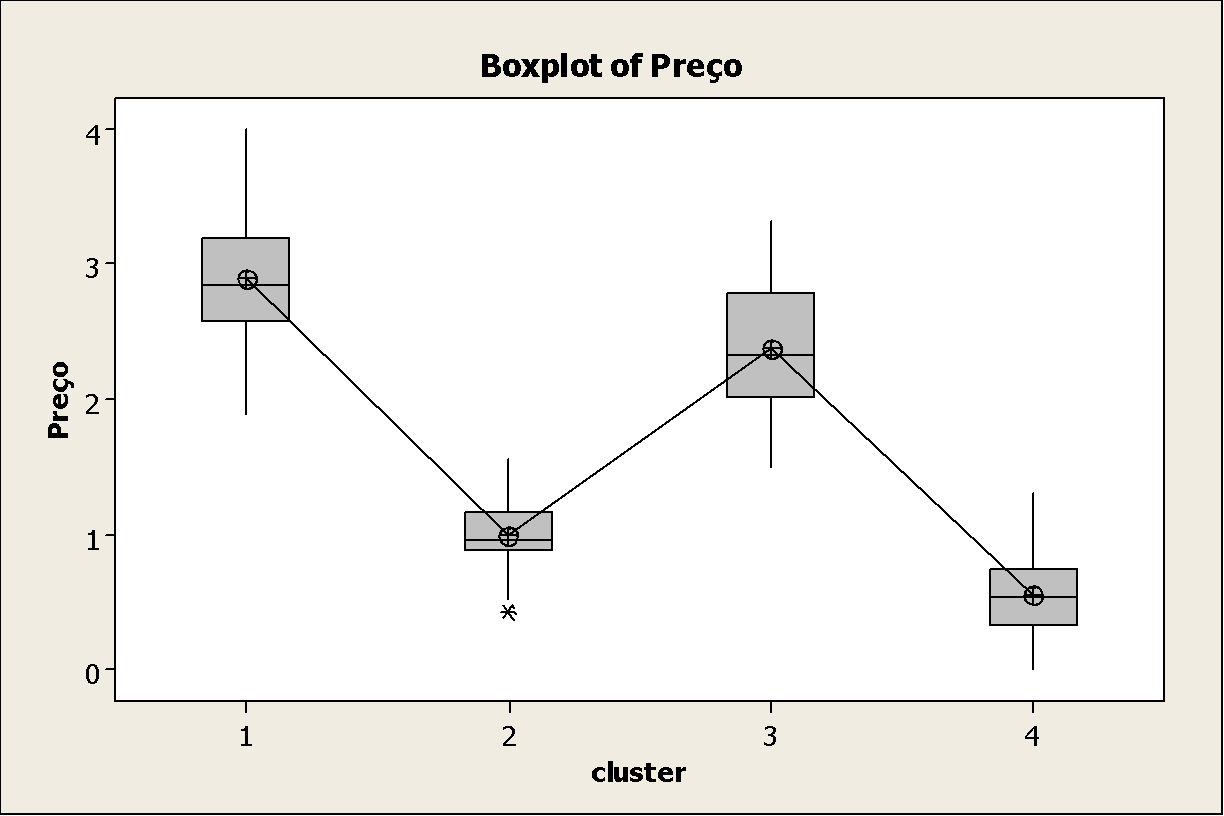
\includegraphics[width=0.45\textwidth]{Imagens/preco_vs_cluster}
\par\end{centering}

}\subfloat[\label{fig:cluster-vs-utilitario}Cluster vs Utilitário: Teste One-way
ANOVA indica Valor $p=0$ e $R_{adj}=86,28\%$]{\begin{centering}
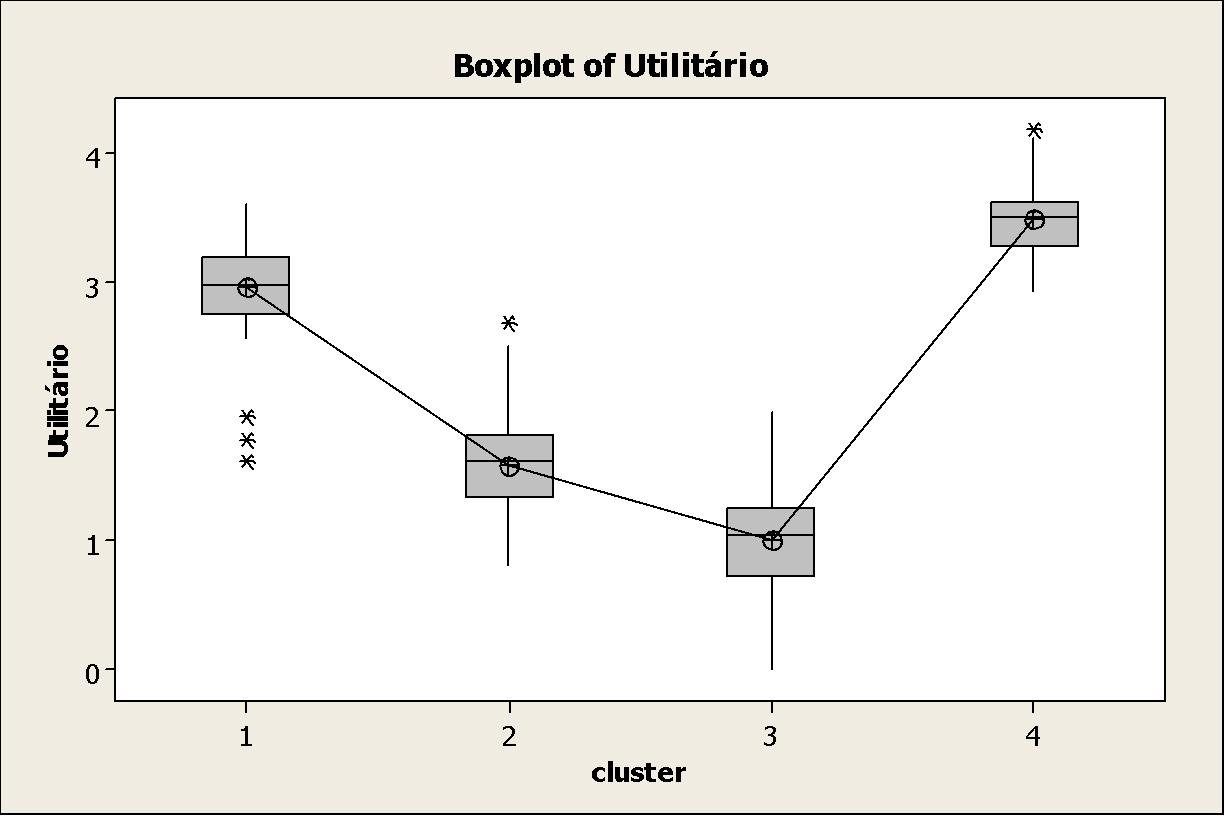
\includegraphics[width=0.45\textwidth]{Imagens/utilitario_vs_cluster}
\par\end{centering}

}
\par\end{centering}

\begin{centering}
\subfloat[\label{fig:boxplot-cluster-vs-imagem}Cluster vs Imagem: Teste One-way
ANOVA indica Valor $p=0$ e $R_{adj}=89,87\%$]{\begin{centering}
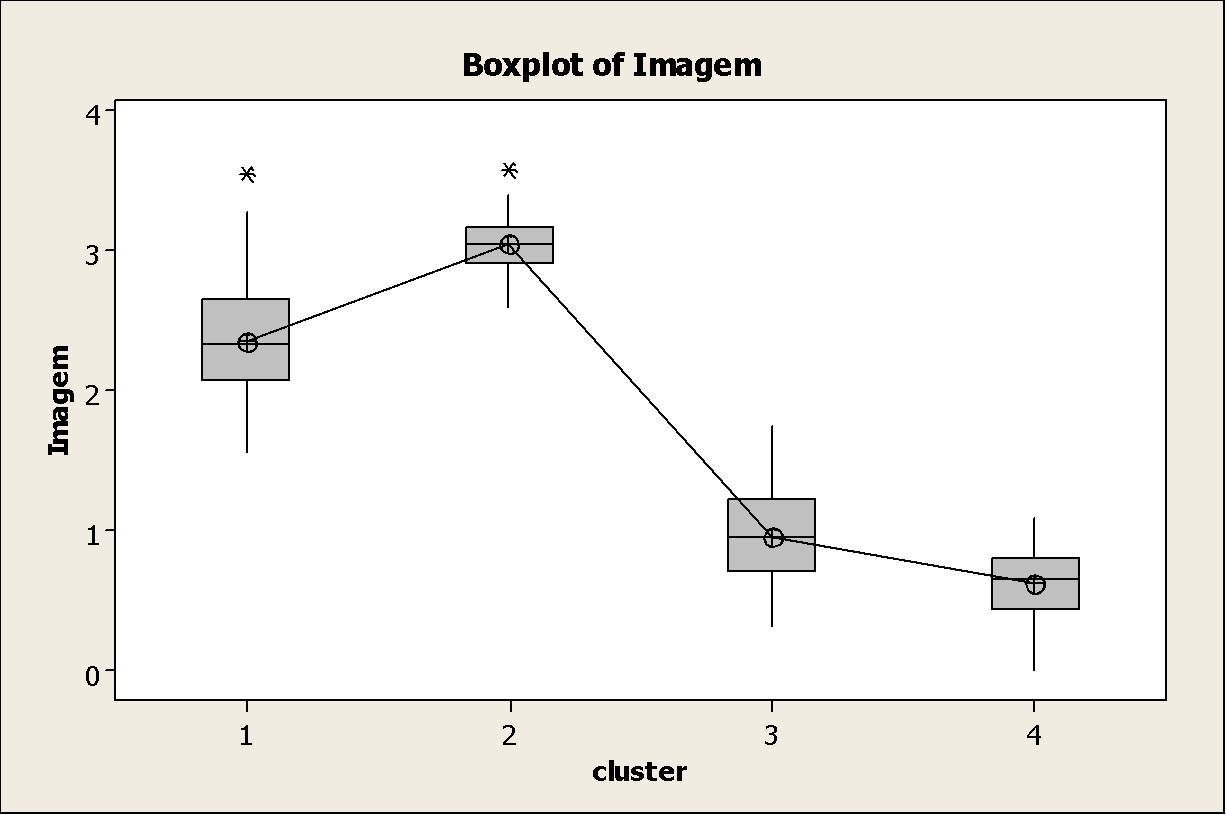
\includegraphics[width=0.45\textwidth]{Imagens/imagem_vs_cluster}
\par\end{centering}

}
\par\end{centering}

\caption{Gráficos de boxplot de variáveis vs \emph{Cluster}}
\end{figure}

\subsection{Imagem}

A imagem é um elemento de marketing mais associado ao marketing transformativo,
e sendo assim, mais voltada para o fator emocional do indivíduo. O
cluster \emph{\nomeCb{}} possui uma forte relação com essa variável,
demonstrado visualmente pelo boxplot da figura \ref{fig:boxplot-cluster-vs-imagem}
e também pelo teste one-way ANOVA do mesmo, com valor $p=0$ e a correlação
$R_{adj}=89,87\%$.

Nos clusters \emph{\nomeCc{}} e \emph{\nomeCd{}} existe uma forte
\emph{reprovação} a imagem o que pode indicar que uma campanha publicitária
focada só nesse fator seria \emph{reprovada} por uma parcela significativa
da população, constituídas pelos clusters mencionados, cuja soma representa
mais de 30\% de todo o espaço amostral.

Tendo isso em vista, apesar do protótipo 3 possuir forte correlação
com o grupo dos \emph{\nomeCb{}}, parece que uma propaganda baseada
nesse protótipo seria pouco abrangente nos clusters mencionados anteriormente. 

\subsection{Preço}

O teste t-Student para o preço tem valor $p=0$, indicando que há também relação
entre o preço e os clusters. Na figura \ref{fig:cluster-vs-preco},
demonstra-se que os clusters \emph{\nomeCa{}} e o \emph{\nomeCc{}}
seguem o indicador preço, enquanto o mesmo não pode ser dito nos
clusters \emph{\nomeCb{}} e \emph{\nomeCd{}}. Isso pode indicar que o preço não
é um fator decisivo na compra desses últimos, e uma estratégia publicitária
para eles não envolve o apelo popular (custo) do carro.

Já para o cluster dos \emph{\nomeCc{}}, o único apelo possível é a questão
popular, isto é, é um cluster que não se relaciona com as outras variáveis
alvos deste estudo.

\subsection{Utilitário}

O fator utilitário quando testado com relação ao cluster, indica por
meio do teste t-Student um valor $p=0$ e pelo boxplot, figura \ref{fig:cluster-vs-utilitario},
indica maior relação com o cluster \emph{\nomeCd{}} e com o cluster
\emph{\nomeCa{}}. 

Os \emph{\nomeCd{}} são o menor dos clusters em número total de amostras,
indicando que uma campanha informativa, voltada para as questões utilitárias
do veículo seria eficaz nesse grupo. Entretanto, focar nele seria
atingir uma pequena parcela do espaço amostral. Já os \emph{\nomeCa{}},
apresentam características mais heterogêneas, incluindo uma relação
estreita com Imagem, tornando uma abordagem meramente informativa
de marketing não eficaz em seu caso. 

\begin{table*}
\begin{centering}
\begin{tabular}{c|c|c|c|c|c}
\hline 
Gênero/Cluster & \nomeCa{} & \nomeCb{} & \nomeCc{} & \nomeCd{} & Todos\tabularnewline
\hline 
Feminino & 25,64 & 34,62 & 74,19 & 81,25 & 47,60\tabularnewline
\hline 
Masculino & 74,36 & 65,38 & 25,81 & 18,75 & 52,40\tabularnewline
\hline 
\emph{Total} & 100 & 100 & 100 & 100 & 100\tabularnewline
\hline 
\end{tabular}
\par\end{centering}

\caption{\label{tab:genero-vs-cluster}Tabela de Análise Chi-quadrado ($\chi^{2}=52,45$;$DF=3$)
Gênero x Cluster. Valor $p=0$.}
\end{table*}

\subsection{Gênero}

A tabela \ref{tab:genero-vs-cluster}, demonstra a dispersão de gênero
ao longo dos clusters sob a perspectiva da análise Chi-quadrado. Para
essa análise, o valor p encontrado é 0, indicando que há correlação
entre gênero e cluster. 

\begin{figure}[h]
\begin{centering}
\subfloat[\label{fig:genero-vs-utilitario}Genero vs Utilitário: Teste t-Student com
$p=0,23$.]{\begin{centering}
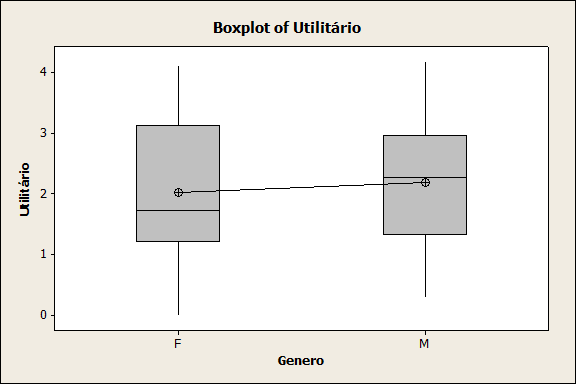
\includegraphics[width=0.45\textwidth]{Imagens/genero_vs_utilitario}
\par\end{centering}

}\subfloat[\label{fig:genero-vs-preco}Gênero vs Preço: Teste t-Student com $p=0,01$.]{\begin{centering}
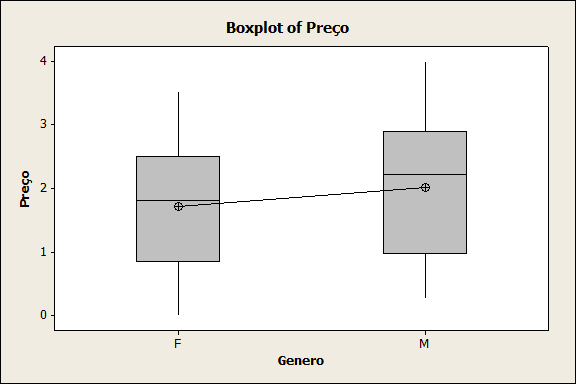
\includegraphics[width=0.45\textwidth]{Imagens/genero_vs_preco}
\par\end{centering}

}
\par\end{centering}

\begin{centering}
\subfloat[\label{fig:boxplot-genero-vs-imagem}Boxplot Gênero vs Imagem: Teste t-Student
com $p=0$.]{\begin{centering}
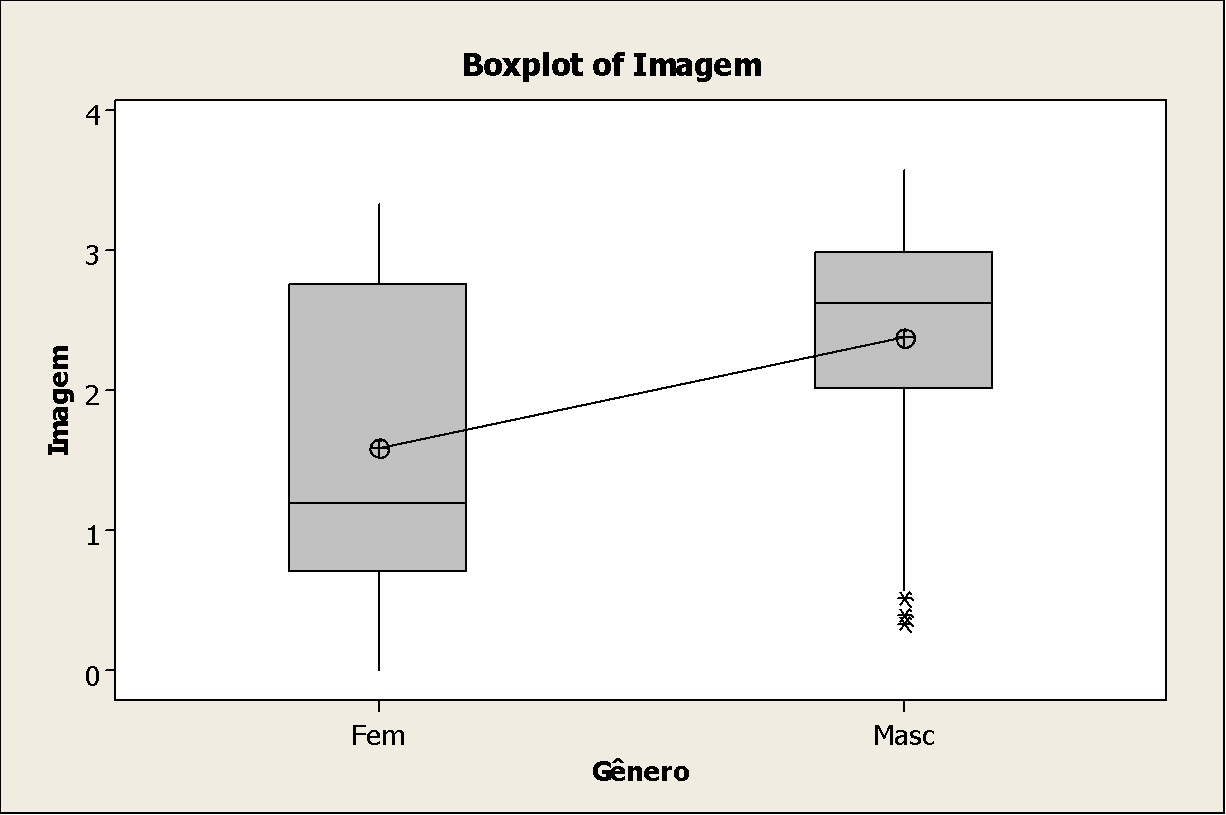
\includegraphics[width=0.45\textwidth]{Imagens/imagem_vs_genero}
\par\end{centering}

}
\par\end{centering}

\caption{Boxplots de Gênero em relação a outras variáveis.}
\end{figure}

Observa-se forte tendência ao gênero \emph{Masculino} nos clusters
\emph{\nomeCa{}} e \emph{\nomeCb{}}, caracterizados sobretudo pela existência
de relação de Imagem com o cluster, e no caso do cluster \emph{\nomeCa{}},
também pela variáveis \emph{Preço} e \emph{Utilitário}.

Quanto ao gênero \emph{Feminino}, tem-se uma maior concentração nos
clusters \emph{\nomeCc{}}, caracterizado por pessoas que não possuem preferência
específica por carros e no cluster \emph{\nomeCd{}}. Podemos assim considerar
que as mulheres da população concentram-se mais no fator \emph{Utilitário}
do protótipo? Não. A figura \ref{fig:genero-vs-utilitario} descarta
essa relação, também demonstrada pelo teste t-Student da relação,
cujo valor $p=0,23$ indica que a hipóteste nula, $H_{0}$, é aceita.


\subsubsection{Gênero e Preço}

O teste t-Student para \emph{Gênero} e \emph{Preço} obtém $p=0,01$ o que indica
correlação entre ambos. A relação em questão é, conforme vista na
figura \ref{fig:genero-vs-preco}, uma relação \emph{negativa} entre
o gênero \emph{Feminino} e a variável \emph{Preço}. Conclui-se que
as mulheres ligam menos para o aspecto \emph{Preço} do carro que os
homens para essa amostra. 

Sabe-se que uma campanha publicitária com foco em \emph{Preço} atingiria
diretamente o grupo dos \emph{\nomeCc{}} que é um dos grupos mais
homogêneos. Entretanto, o fato de haver um fator de indiferença do
gênero feminino para essa variável dificulta mais ainda o marketing
focado para um gênero. Ainda mais que na figura mencionada, vê-se
que a variável \emph{Preço} possui grande variabilidade no gênero masculino.
Conclui-se que uma publicidade informativa voltada a \emph{Preço} além
de dificultosa, seria pouco eficaz no que toca \emph{Gênero}.


\subsubsection{Gênero e Imagem}

Sabendo-se que há relação de \emph{Gênero} e \emph{Cluster}, podemos assim focar
parcialmente a estratégia de propaganda em gêneros, podendo assim
veicular em meios mais associados ao gênero em questão. 

Por exemplo, assumindo-se que o público feminino que assiste jogos
do campeonato brasileiro seja inferior ao masculino, faria sentido
veicular uma propaganda do cluster \emph{\nomeCc{}} ou do cluster
\emph{\nomeCd{}} no intervalo das partidas do mesmo? Pouco provável,
por isso o gênero pode ser fator determinante na estratégia adotada
de marketing para a campanha publicitária do protótipo.

Para tirar-se a questão a limpo, basta olhar o boxplot de imagem em
função ao gênero, da figura \ref{fig:boxplot-genero-vs-imagem}, onde
há uma forte associação ao gênero masculino nas notas mais altas de
imagem, indicando que uma estratégia de marketing para imagem, deve
provavelmente levar o gênero em consideração. Aplicando-se o teste t-Student
na amostra, obtêm-se um valor $p=0$, elucidando assim
que aceita-se $H_{a}$ na análise de ambos.

\begin{center}
\begin{table*}
\begin{centering}
\begin{tabular}{c|c|c|c|c|c}
\hline 
Filhos/Cluster & \nomeCa & \nomeCb & \nomeCc & \nomeCd & Todos\tabularnewline
\hline 
Não & 53,85 & 60,26 & 74,19 & 50 & 60,40\tabularnewline
\hline 
Tem & 46,15 & 39,74 & 25,81 & 50 & 39,60\tabularnewline
\hline 
\emph{Total} & 100 & 100 & 100 & 100 & 100\tabularnewline
\hline 
\end{tabular}
\end{centering}
\caption{\label{tab:filhos-vs-cluster}Tabela de Análise Chi-quadrado ($\chi^{2}=7,78$;$DF=3$),
Filhos x Cluster. Valor $p=0,05$.}
\end{table*}
\end{center}

\subsection{Filhos}

A tabela \ref{tab:filhos-vs-cluster}, demonstra a dispersão de gênero
ao longo dos clusters sob a perspectiva da análise Chi-quadrado. Para
essa análise, o valor $p=0,05$. Ou seja, há relação entre ter filhos
e cluster. 

Sabe-se também que o valor p para o Chi-quadrado de \emph{Estado Civil}
vs \emph{Clusters} indica é $0,96$. Isto é, a hipótese $H_{0}$ é
aceita, e não há relação entre ambos. Sendo assim, conclui-se que
independente do estado civil, há uma questão importante a ser abordada
na campanha publicitária: possui ou não filhos.

Os clusters \emph{\nomeCb{}} e \emph{\nomeCc{}} possuem uma população majoritariemente
sem filhos, enquanto os \emph{\nomeCa{}} e \emph{\nomeCd{}} são ``meio a meio''. 

A existência dessa variável pode então influenciar parcialmente uma
publicidade direcionada, principalmente para um marketing transformativo.

\begin{center}
\begin{table*}
\begin{centering}
\begin{tabular}{c|c|c|c|c|c}
\hline 
Pequeno/Cluster & \nomeCa & \nomeCb & \nomeCc & \nomeCd & Todos\tabularnewline
\hline 
Não & 73,08 & 76,92 & 100 & 75 & 81,20\tabularnewline
\hline 
Sim & 26,92 & 23,08 & 0 & 25 & 18,80\tabularnewline
\hline 
\emph{Total} & 100 & 100 & 100 & 100 & 100\tabularnewline
\hline 
\end{tabular}
\end{centering}

\caption{\label{tab:tamanho-vs-cluster}Tabela de Análise Chi-quadrado ($\chi^{2}=19,47$;$DF=3$),
Prefere Carro Pequeno vs Cluster. Valor $p=0,0$.}
\end{table*}
\end{center}

\subsection{Prefere Carro Pequeno}


O tamanho do carro é um fator importante de marketing? Sim, porque
na tabela \ref{tab:tamanho-vs-cluster} há uma intensa relação entre
as variáveis \emph{Carro Pequeno} e \emph{Cluster}.

Para os \emph{\nomeCc{}} e \emph{\nomeCd{}} há predominância daqueles que não
gostariam de um carro pequeno, enquanto nos clusters \emph{\nomeCa{}} e
\emph{\nomeCb{}} é o oposto. 

Especialmente no cluster \emph{\nomeCc{}} a relação é tão forte que não
há preferência por carros pequenos. Então, uma campanha transformativa
para esses grupos deve levar em consideração o espaço do carro, uma
vez que há relação entre ambos.



% ----------------------------------------------------------
% Finaliza a parte no bookmark do PDF
% para que se inicie o bookmark na raiz
% e adiciona espaço de parte no Sumário
% ----------------------------------------------------------
\phantompart

% ---
% Conclusão - Recomendação de qual protótipo
% ---
\chapter{Recomendação de Campanha para Protótipo}
% ---

%Placeholder
\label{chap:conclusao}

\begin{figure}
\begin{centering}
\subfloat[\label{fig:prototipo-familia}Conforto,
espaço e filhos.]{\begin{centering}
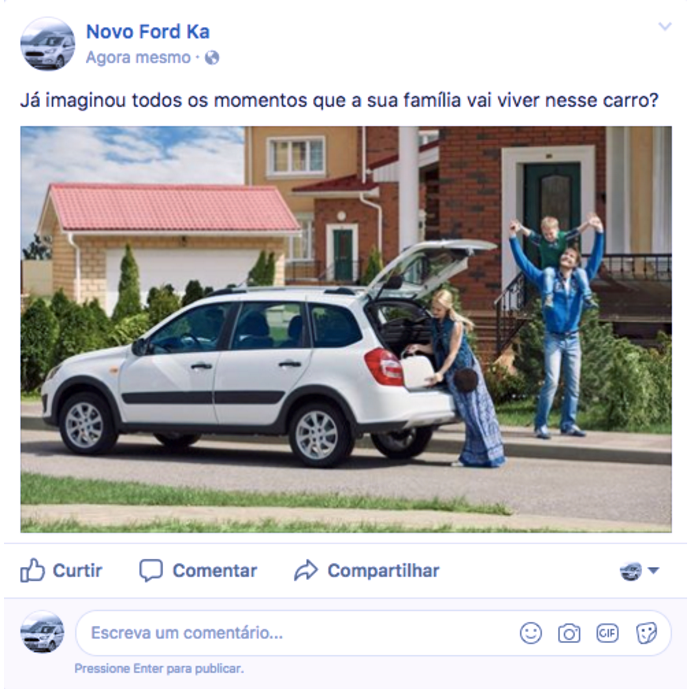
\includegraphics[height=0.30\textheight]{Imagens/p1_familia}~~
\par\end{centering}
}\subfloat[\label{fig:prototipo-versatil}Aborda o efeito versátil do carro.]{\begin{centering}
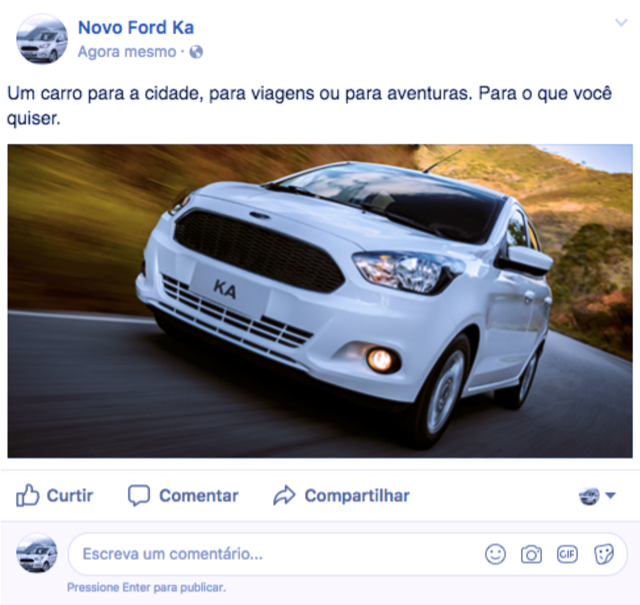
\includegraphics[height=0.30\textheight]{Imagens/p1_prototipo}
\par\end{centering}
}
\par\end{centering}
\caption{Peças ilustrativas de uma campanha em formato carrossel.}
\end{figure}

De acordo com o desenvolvido no capítulo \ref{chap:analise}, com
as tabelas \ref{tab:prototipo-vs-cluster} e \ref{tab:prototipo-analise},
contrasta a homogeneidade dos protótipo 2 e 3 à heterogeneidade do
protótipo 1. À primeira vista, percebe-se que os três protótipos possuem
proporções da população muito parecidas, entretanto há uma grande
diferença entre o protótipo 1, heterogêneo, com os demais protótipos.
Isto é, a possibilidade de uma campanha publicitária informativa unida
a transformativas que possibilitarão, se escolhido o protótipo 1,
abranger também os clusters \nomeCc{} e \nomeCb{}, dado que pela
própria heterogeneidade do protótipo 1, certas propagandas que apelam
para determinadas características do protótipo podem aumentar a aceitação
de uma campanha baseada neste protótipo.

\begin{table}
\begin{centering}
\begin{tabular}{c|>{\centering}p{0.28\textwidth}|>{\centering}p{0.28\textwidth}|>{\centering}p{0.28\textwidth}}
\hline 
 & Protótipo 1 & Protótipo 2 & Protótipo 3\tabularnewline
\hline 
Bom & Preferido entre \nomeCa{} e \nomeCd{}. & Amplamente preferido pelo cluster dos \nomeCc{}. & Amplamente preferido pelos \nomeCb{}, focados em Imagem.\tabularnewline
\hline 
Ruim & Somente uma estratégia de marketing não é suficiente, dada a sua heterogeneidade
e várias afinidades. & Difícil para a publicidade porque se mostra indiferente a carros.
Importam-se apenas com o preço. & Uma campanha publicitária em Imagem somente não gera interesse de
outros clusters.\tabularnewline
\hline 
\end{tabular}
\par\end{centering}
\caption{\label{tab:prototipo-analise}Vantagens e desvantagens por protótipos.}
\end{table}


Por exemplo, se uma campanha publicitária apelar de maneira informativa
e transformativa para os aspectos de Imagem e Utilitário do carro,
é possível abranger os clusters mencionados anteriormente, sustentando
assim uma aceitação maior por parte da população. Ou seja, escolhe-se
a versatilidade do protótipo 1, numa eventual campanha publicitária
como elemento.

\begin{figure}
\begin{centering}
\subfloat[\label{fig:painel-cambio}Acabamento e câmbio.]{\begin{centering}
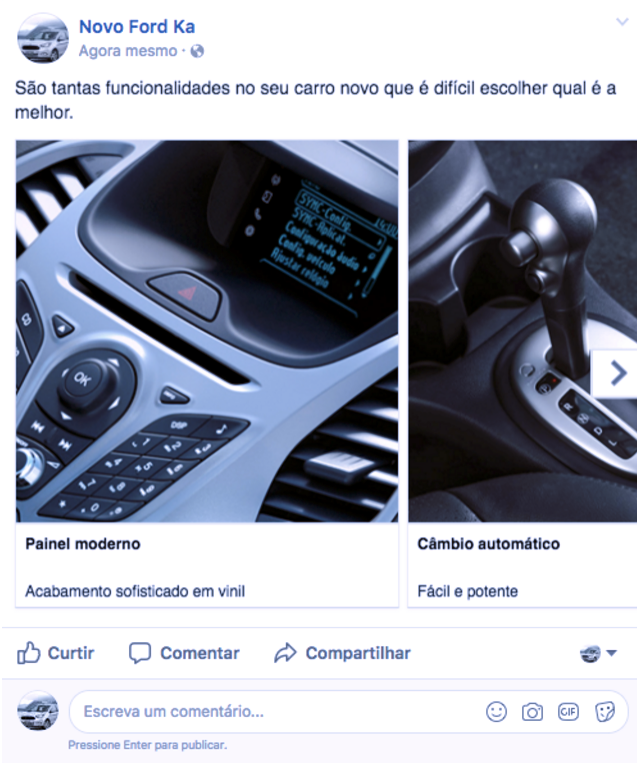
\includegraphics[height=0.34\textheight]{Imagens/p1_interior}
\par\end{centering}
}~~\subfloat[\label{fig:ar}Ar-condicionado.]{\begin{centering}
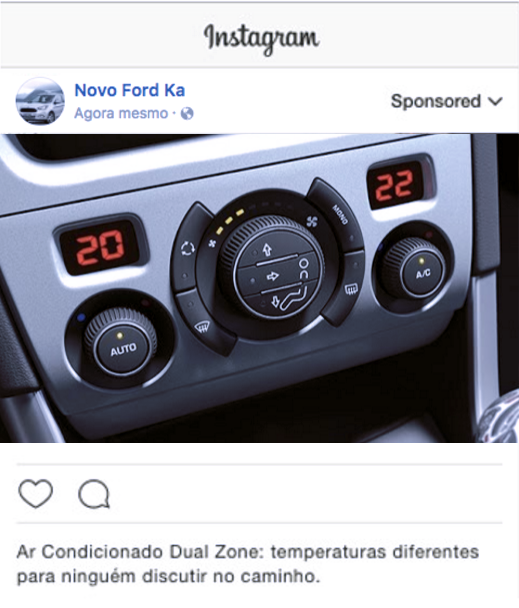
\includegraphics[height=0.34\textheight]{Imagens/p1_interior_painel}
\par\end{centering}
}
\par\end{centering}
\caption{Peças multifuncionais para Utilitário e Imagem.}
\end{figure}


\section{Recomendações para Campanha Publicitária}

Com base nas características analisadas dos grupos \nomeCa{} e \nomeCd{}
será feita uma combinação de campanhas publicitárias: para os \nomeCa{},
uma campanha transformativa mesclando os três atributos: Imagem, Utilitário
e Preço. Para os \nomeCd{}, uma campanha ressaltando o carro como
utilitário. Por se tratar de dois grupos diferentes vamos destacar
multifuncionalidade, tecnologia, versatilidade e conforto.

É possível uma campanh que foque nas seguintes características: confortável
e espaçoso. O público-alvo seriam os \nomeCd{} que preferem carros
como bens utilitários, destacando o porta-malas espaçoso para a família.
Os \nomeCd{} são formados predominantemente por mulheres com filhos,
por isso o destaque a família, na figura \ref{fig:prototipo-familia}.

A campanha com formato em carrossel irá abordar a característica de
multifuncionalidade. A publicidade tem foco nos \nomeCa{} combinando
funcionalidades (Utilitário) que valorizem o carro (Preço) e que tragam
mais sofisticação (Imagem), como vê-se nas figuras \ref{fig:painel-cambio}
e \ref{fig:ar}.

Finalmente, a figura \ref{fig:prototipo-versatil} seria veiculada
em formato vídeo, tanto em Facebook quanto na televisão. Destaca a
versatilidade do Ford Ka\texttrademark, valorizando o fato de ser
um carro potente (Utilitário) e ainda assim econômico (Preço). Em
televisão, dá-se preferência é por intervalos de jogos de futebol
buscando atingir um público predominantemente masculino que gosta
de esportes e aventuras. 



% ----------------------------------------------------------
% ELEMENTOS PÓS-TEXTUAIS
% ----------------------------------------------------------
\postextual
% ----------------------------------------------------------

% ----------------------------------------------------------
% Referências bibliográficas
% ----------------------------------------------------------
\bibliography{referencias}

% ----------------------------------------------------------
% Glossário
% ----------------------------------------------------------
%
% Consulte o manual da classe abntex2 para orientações sobre o glossário.
%
%\glossary

% ----------------------------------------------------------
% Apêndices
% ----------------------------------------------------------

% ---
% Inicia os apêndices
% ---
%\begin{apendicesenv}

%% Imprime uma página indicando o início dos apêndices
%\partapendices

%% ----------------------------------------------------------
%\chapter{Quisque libero justo}
%% ----------------------------------------------------------

%\lipsum[50]

%% ----------------------------------------------------------
%\chapter{Nullam elementum urna vel imperdiet sodales elit ipsum pharetra ligula
%ac pretium ante justo a nulla curabitur tristique arcu eu metus}
%% ----------------------------------------------------------
%\lipsum[55-57]

%\end{apendicesenv}
% ---


% ----------------------------------------------------------
% Anexos
% ----------------------------------------------------------

% ---
% Inicia os anexos
% ---
%\begin{anexosenv}

%% Imprime uma página indicando o início dos anexos
%\partanexos

%% ---
%\chapter{Morbi ultrices rutrum lorem.}
%% ---
%\lipsum[30]

%% ---
%\chapter{Cras non urna sed feugiat cum sociis natoque penatibus et magnis dis
%parturient montes nascetur ridiculus mus}
%% ---

%\lipsum[31]

%% ---
%\chapter{Fusce facilisis lacinia dui}
%% ---

%\lipsum[32]

%\end{anexosenv}

%---------------------------------------------------------------------
% INDICE REMISSIVO
%---------------------------------------------------------------------
\phantompart
\printindex
%---------------------------------------------------------------------

\end{document}
